
\begin{figure}[!htbp]
    \centering
    \begin{subfigure}[b]{0.5\textwidth}
      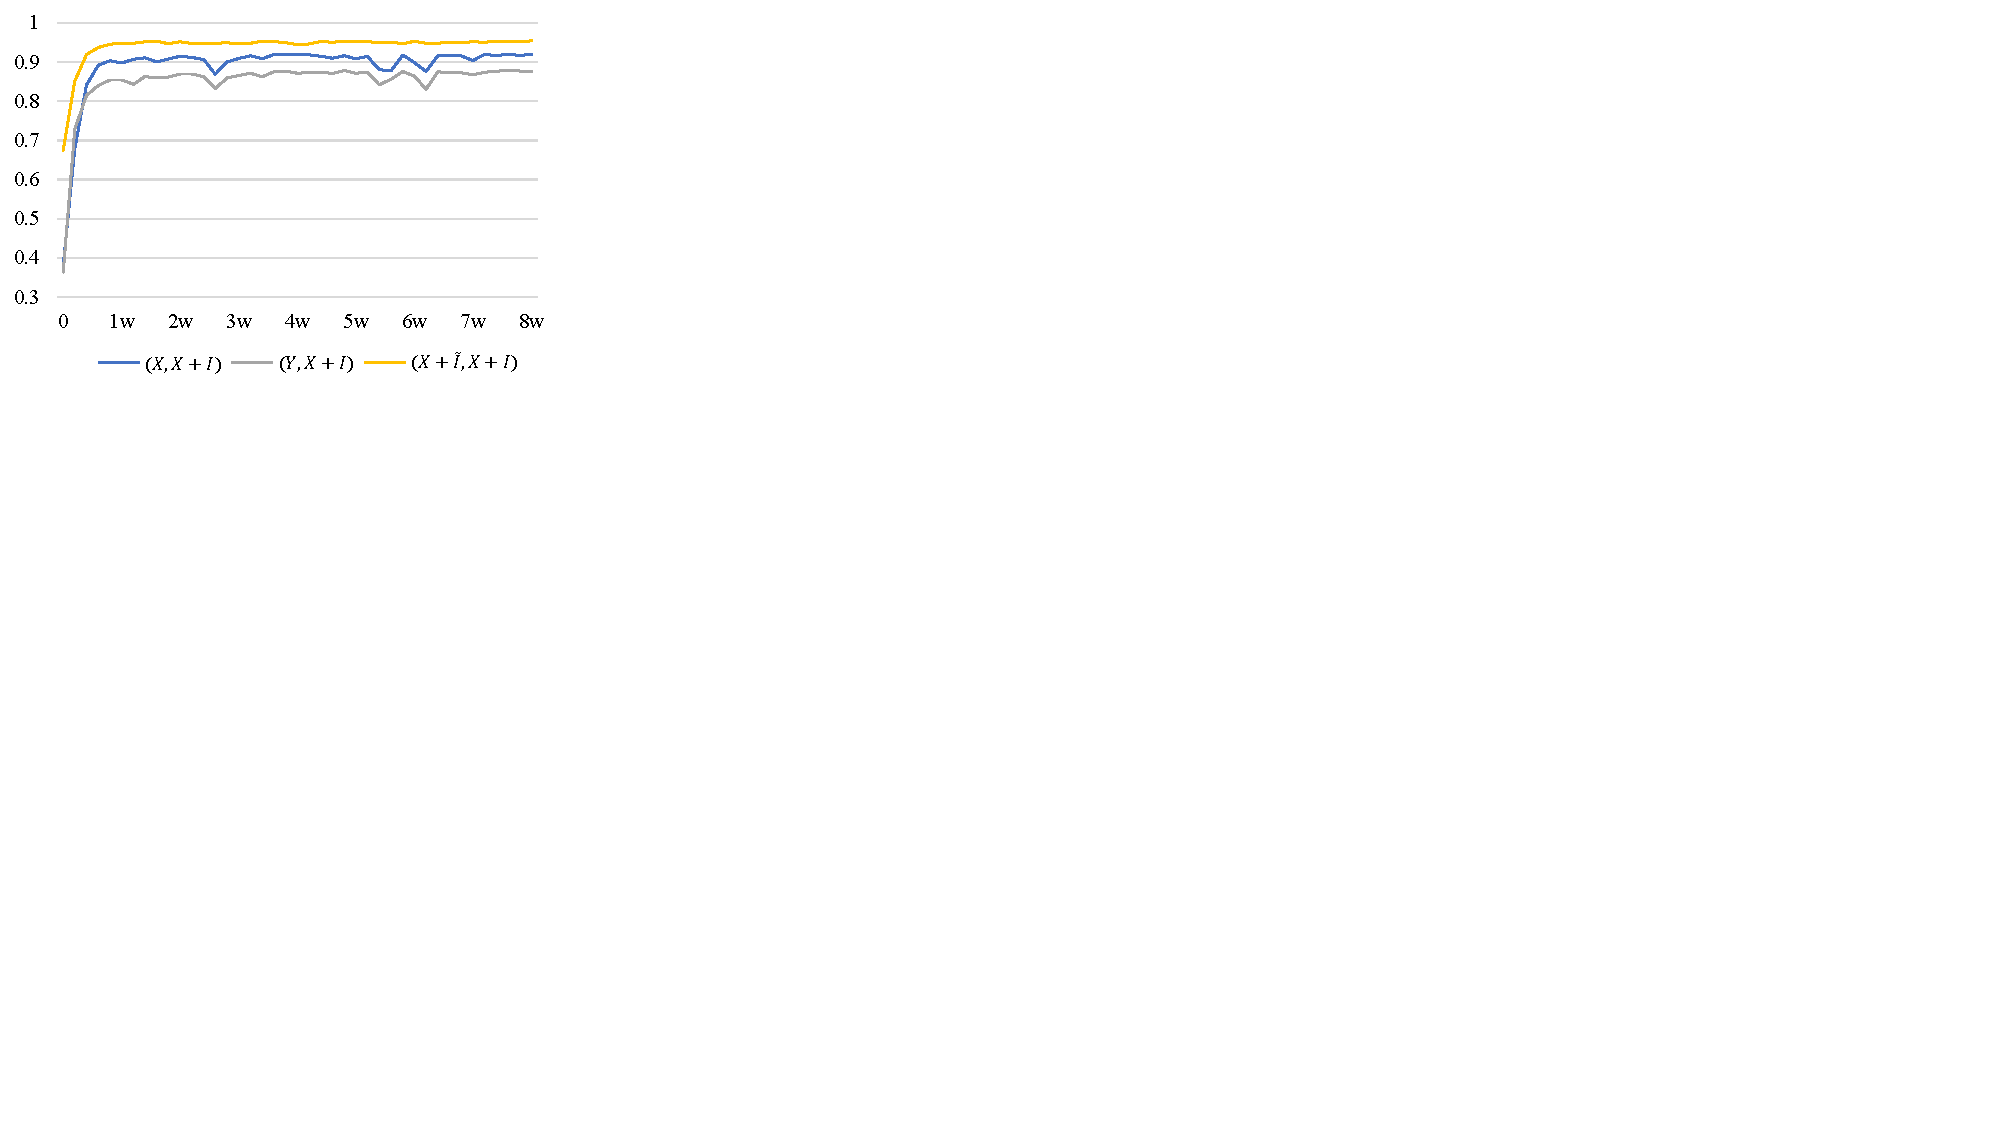
\includegraphics[width=\textwidth]{Img/fig_5_training_cat_mmt_bi.pdf}
      \caption{CAT-NMT~+~BDTT}
      \label{fig:5_training_cat_mmt_bi}
    \end{subfigure}%
    ~% add desired spacing
    \begin{subfigure}[b]{0.5\textwidth}
      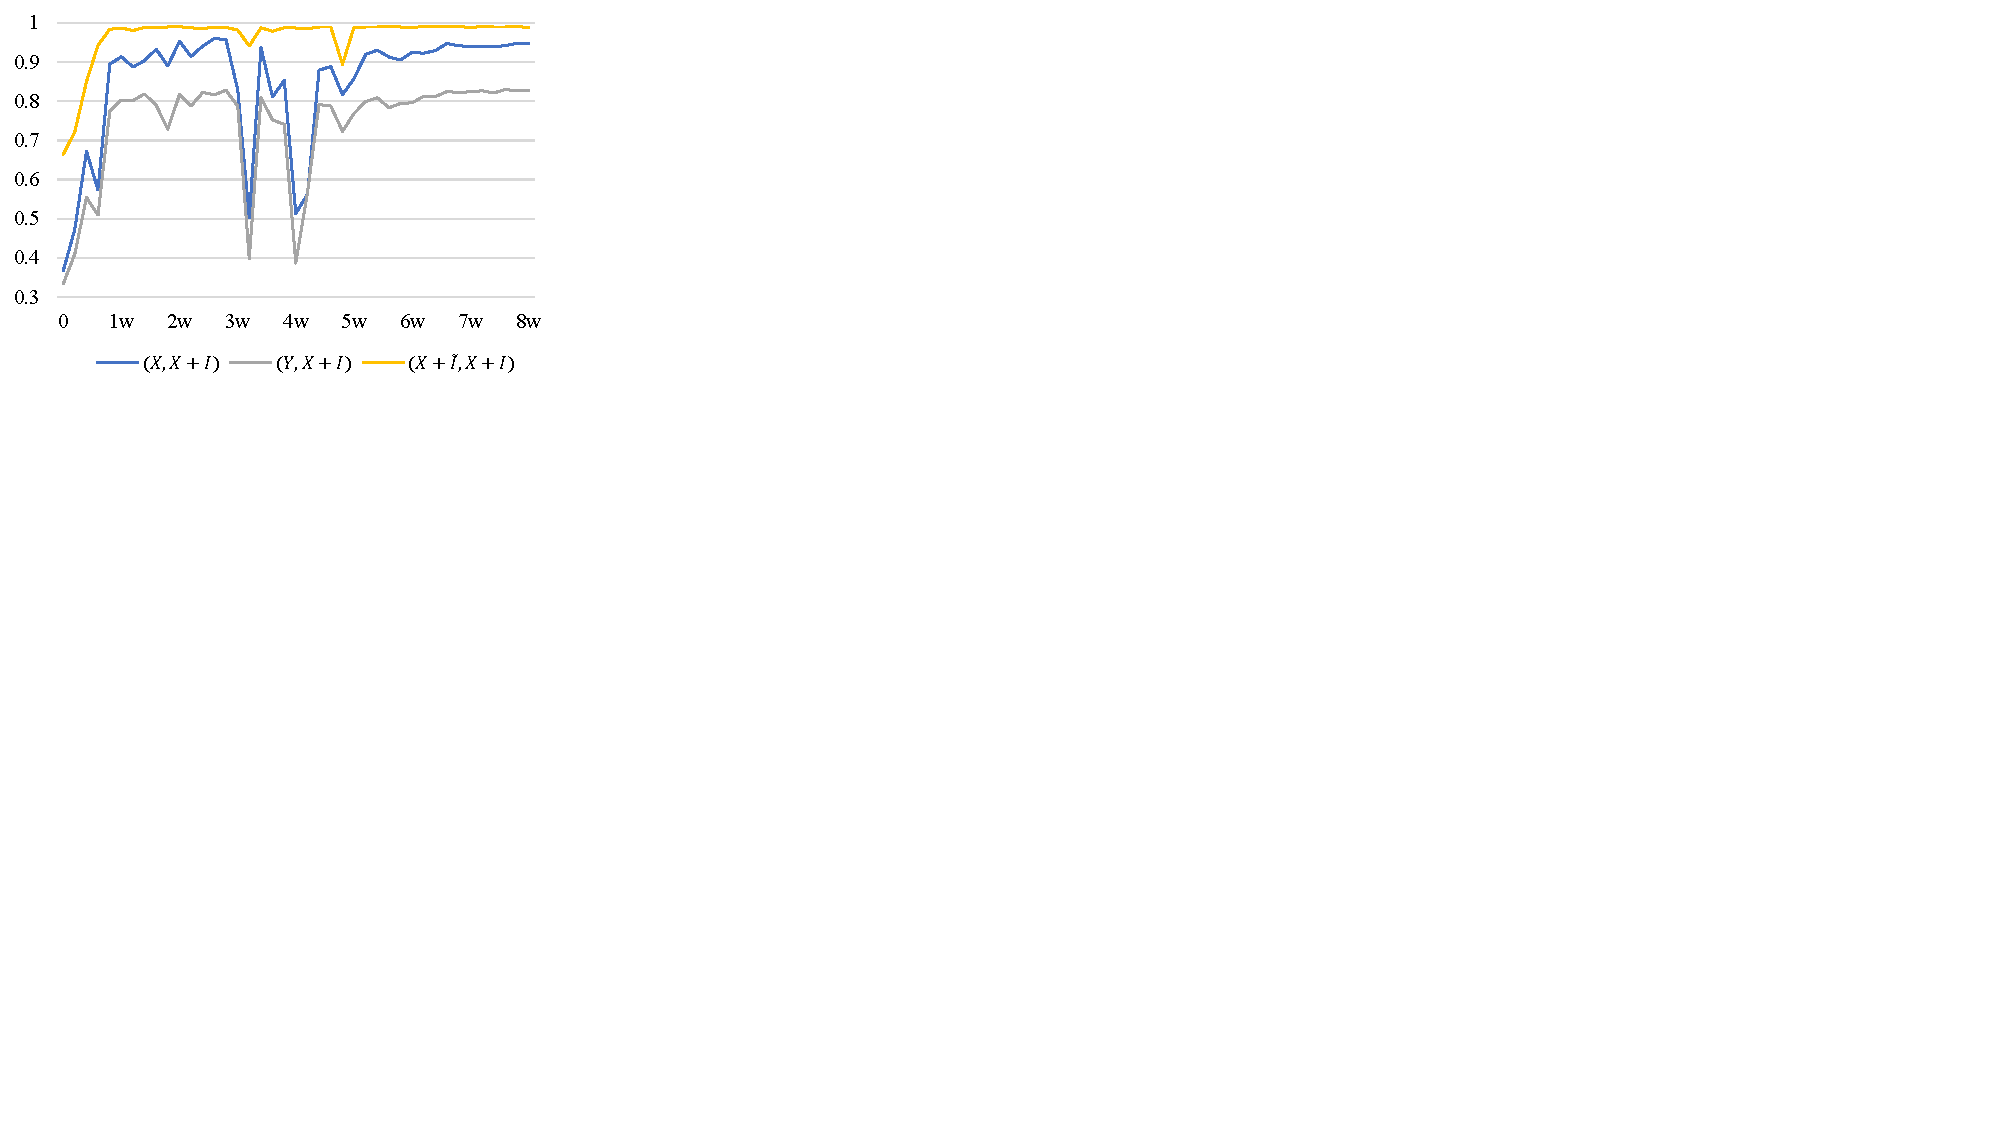
\includegraphics[width=\textwidth]{Img/fig_5_training_cat_mmt.pdf}
      \caption{CAT-NMT}
      \label{fig:5_training_cat_mmt}
    \end{subfigure}
    \bicaption{双向翻译训练方法在模型训练过程中对样本余弦距离的影响}{Influence of BDTT on cosine distance among samples during model training}
    \label{fig:5_training}
\end{figure}